\documentclass[a4paper,11pt]{article}
\usepackage{graphicx}
\usepackage[margin=1in]{geometry}

\usepackage[table,xcdraw]{xcolor}
\usepackage[utf8]{inputenc}
\usepackage{ulem}
\usepackage{color}
\usepackage{enumerate}
\usepackage{amssymb}
\usepackage{amsmath}
\usepackage {tikz}
\usetikzlibrary{arrows,matrix,positioning}
%\usepackage{bera}
\usepackage{listings}
\usepackage{xcolor}
\usepackage{framed}
\usepackage[hidelinks]{hyperref}
\usepackage{enumitem}
%\setenumerate[2]{label=\roman*.}
\usepackage{blindtext}
\usepackage{fancyhdr}
\pagestyle{fancy}
\usepackage{hhline}
\colorlet{punct}{red!60!black}
\definecolor{background}{HTML}{EEEEEE}
\definecolor{delim}{RGB}{20,105,176}
\colorlet{numb}{magenta!60!black}

\definecolor {processblue}{cmyk}{0.96,0,0,0}

%\setenumerate[1]{label=\textbf{\thesection.\arabic*.}}


\begin{document}
\textbf{Integration of 1-forms on Graphs}

\bigskip

\textbf{Introduction}

\bigskip

Given a connected graph $G=(V,E)$ with $V$ vertices, and $E$ edges and a 
1-form $v: E \rightarrow \mathbb{R}^D$. We 're looking for the 0-form 
$x: V \rightarrow \mathbb{R}^D$ minimizing the error:

$$E(x) = \sum_{(i,j) \in E} ||dx_{ij} - v_{ij}||^2$$

where $dx: E \rightarrow \mathbb{R}^D$ is the differential of $x$.

\bigskip

\textbf{Obs. 1}: It is sufficient to consider the case $D=1$, because 
the problem can be reduced to solving $D$ independent 1-D problems on 
the same graph for each coordinate.

\bigskip

\textbf{Obs. 2} (Abuses of notation): We use $V$ to denote both the set 
of vertices and the total number of vertices of the graph. And we denote 
$v$ to the 1-form and $v_i$ is the $i-th$ vertex.

\bigskip

\textbf{Obs. 3}: Vertices and edges can be enumerated in many different 
ways. We will enumerate vertices and edges according to a traversal 
order of a spanning tree. This process determine a consistent 
orientation of the edges: an edge will be oriented from a lower vertex 
to a greater vertex:

$$e_{ij}: v_i \rightarrow v_j \ (for \ i < j)$$

\bigskip

\textbf{Integration process}

\bigskip

The proposed process for integrating $v$ is as follows:

\begin{enumerate}
	\item Construct a spanning tree $T$ for $G$
	\item Choose an order of traversal for $T$ and orient the edges 
	from parent to child
	\item Enumerate the vertices and tree edges according to the order 
	of traversal (See figure~\ref{fig:M1})
	\item We will refer to the remaining graph edges (those which do not 
	belong to the tree) as ``loop-edges". Orient the loop-edges from 
	parent to child.
	\item Construct the incidence matrix $D$: this is an $E \times V$ 
	sparse matrix with one row per graph edge and one column per vertex. For 
	each edge $e_{ij} \ (i < j)$ we set the $i-th$ column entry to $-1$ 
	and the $j-th$ column to $1$ (See figure~\ref{fig:M2}).
\end{enumerate}


\begin{figure}
\centering
\begin {tikzpicture}[-latex ,auto ,node distance =3cm ,on grid ,
semithick ,state/.style ={ circle ,top color =white , bottom color = processblue!20 ,
draw,processblue , text=blue , minimum width =1 cm},
edge/.style = {->,> = latex'}]
\node[state] (1) {$1$};
\node[state] (2) [below left=of 1] {$2$};
\node[state] (3) [below  right =of 1] {$3$};
\node[state] (4) [below  left =of 2] {$4$};
\node[state] (5) [below  left =of 3] {$5$};
\node[state] (6) [below  right =of 3] {$6$};
\node[state] (7) [below  left =of 4] {$7$};
\node[state] (8) [below  right =of 4] {$8$};
\node[state] (9) [below  right =of 5] {$9$};
\path (1) edge node {1} (2);
\path (1) edge node {2} (3);
\path (2) edge node {3} (4);
\path (3) edge node {4} (5);
\path (3) edge node {5} (6);
\path (4) edge[red] node {} (5);
\path (4) edge node {6} (7);
\path (4) edge node {7} (8);
\path (5) edge node {8} (9);
\path (8) edge[red] node {} (9);
\end{tikzpicture}

\caption{BFS traversal of a spanning tree. Nodes and edges are 
enumerated according tree traversal. Edges are oriented from 
parent to child. Red edges correspond to 
$loop-edges$.}
\label{fig:M1}
\end{figure}

\begin{figure}
\centering
%$\begin{pmatrix}
%-1 & 1  & 0  & 0  & 0  & 0 & 0 & 0  & 0 &  \\
%-1 & 0  & 1  & 0  & 0  & 0 & 0 & 0  & 0 &  \\
%0  & -1 & 0  & 1  & 0  & 0 & 0 & 0  & 0 &  \\
%0  & 0  & -1 & 0  & 1  & 0 & 0 & 0  & 0 &  \\
%0  & 0  & -1 & 0  & 0  & 1 & 0 & 0  & 0 &  \\
%0  & 0  & 0  & -1 & 0  & 0 & 1 & 0  & 0 &  \\
%0  & 0  & 0  & -1 & 0  & 0 & 0 & 1  & 0 &  \\
%0  & 0  & 0  & 0  & -1 & 0 & 0 & 0  & 1 &  \\
%0  & 0  & 0  & -1 & 1  & 0 & 0 & 0  & 0 &  \\
%0  & 0  & 0  & 0  & 0  & 0 & 0 & -1 & 1 &
%\end{pmatrix}$
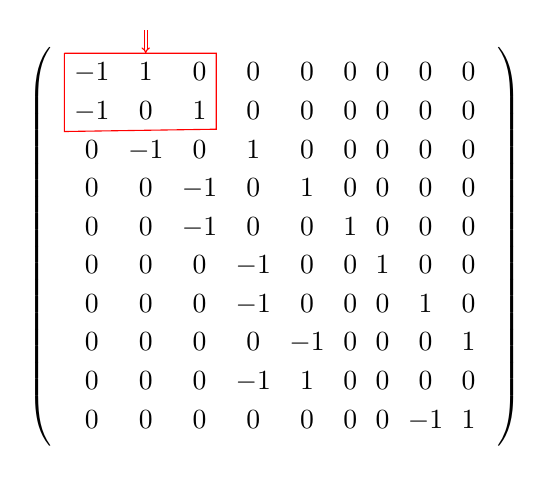
\begin{tikzpicture}
	\matrix [matrix of math nodes,left delimiter=(,right delimiter=)] (m)
	{
		-1 & 1  & 0  & 0  & 0  & 0 & 0 & 0  & 0 &  \\
		-1 & 0  & 1  & 0  & 0  & 0 & 0 & 0  & 0 &  \\
		0  & -1 & 0  & 1  & 0  & 0 & 0 & 0  & 0 &  \\
		0  & 0  & -1 & 0  & 1  & 0 & 0 & 0  & 0 &  \\
		0  & 0  & -1 & 0  & 0  & 1 & 0 & 0  & 0 &  \\
		0  & 0  & 0  & -1 & 0  & 0 & 1 & 0  & 0 &  \\
		0  & 0  & 0  & -1 & 0  & 0 & 0 & 1  & 0 &  \\
		0  & 0  & 0  & 0  & -1 & 0 & 0 & 0  & 1 &  \\
		0  & 0  & 0  & -1 & 1  & 0 & 0 & 0  & 0 &  \\
		0  & 0  & 0  & 0  & 0  & 0 & 0 & -1 & 1 &  \\
	};  
	\draw[color=red] (m-1-1.north west) -- (m-1-3.north east) -- (m-2-3.south east) -- (m-2-1.south west) -- (m-1-1.north west);
	\draw[color=red,double,implies-](m-1-2.north) -- +(0,0.3);
\end{tikzpicture}

\caption{Incidence matrix correspondig to graph in figure~\ref{fig:M1}}
\label{fig:M2}
\end{figure}


\end{document}

